\documentclass[wide,a4paper,titlepage,12pt] {article}
\usepackage{polski}
\usepackage[utf8]{inputenc}
\usepackage{listings}
\usepackage{slashbox}
\usepackage[table]{xcolor}
\usepackage{graphicx,pdflscape}
\usepackage{placeins}

\title{Układy cyfrowe i systemy wbudowane}
\author{Tymon Tobolski (181037)\\ Jacek Wieczorek (181043)}

% Title page layout (fold)
\makeatletter
\renewcommand{\maketitle}{
\begin{titlepage}
  \begin{center}
    \vspace*{3cm}
    \LARGE \@title \par
    \vspace{2cm}
    \textit{\small Autor:}\par
    \normalsize \@author\par \normalsize
    \vspace{3cm}
    \textit{\small Prowadzący:}\par
    Dr inż. Jarosław Sugier \par
    \vspace{2cm}
    Wydział Elektroniki\\ III rok\\ Pn 14.15 - 16.00\par
    \vspace{4cm}
    \small \@date
  \end{center}
\end{titlepage}
}
\makeatother

\begin{document}
\maketitle
  \section{Zadanie nr 1}
  Celem zadania było zamodelowanie układu detektora sekwencji 1 1 0 0 0 przy pomocy automatu Mealy'ego, przetestowanie jego działania w symulatorze, a następnie uruchomienie go na płycie $ZL-9572$. Układ miał za zadanie zapalić diodę LED w momencie wykrycia sekwencji.

  \begin{figure}[htbp]
    \begin{center}
      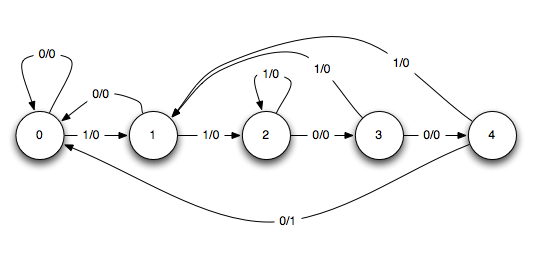
\includegraphics[scale=0.7]{mealy-graf.png}
      \caption{Graf automatu Mealy'ego}
     \end{center}
  \end{figure}


  W celu wyznaczenia odpowiednich kombinacji syngałów dla wejść przerzutników zostosowana została metoda siatek Karnaugh.


  TODO - siatki

Następnym etapem ćwiczenia było napisanie testów oraz odpowiednie zmoodyfikownanie pliku \textit{ZL-9572.ucf} pozwalające na zasymulowanie układu.

  \newpage
  \paragraph{}
  Testy napisane w języku \textit{VHDL}
  \lstinputlisting[language=Vhdl]{code1.txt}

  Kolejnym etapem zadania było zamodelowanie działania schematu za pomocą programu ModelSim oraz zaprogramowanie urządzenia za pomocą złącza \textit{JTAG}.


  \section{Zadanie nr 2}
  Drugim zadaniem było przerobienie automatu z zadania pierwszego na automat Moore'a.

    \begin{figure}[htbp]
    \begin{center}
      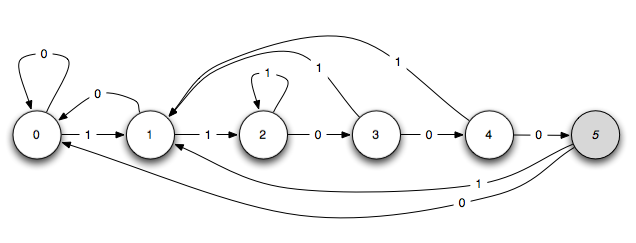
\includegraphics[scale=0.7]{moore-graf.png}
      \caption{Graf automatu Moore'a}
     \end{center}
  \end{figure}



\end{document}



